%!TEX root = ../bericht.tex

\section{Einleitung}

eee

\section{Methoden}


	\subsection{Konzept}
	
		In der Entwicklung einer Osteosyntheseplatte sollen unterschiedliche Aspekte.
		Darunter fallen folgende Aspekte:
		
		\begin{enumerate}
			\setlength{\itemsep}{0mm}
			\setlength{\parskip}{1mm}
			\item Möglichst Minimal-Invasive Technik um Weichteile nicht zu verletzen
		\end{enumerate}
		
		Da meine CAD Konstruktions-Fähigkeiten beschränkt sind 	


\section{Resultate}

	\subsubsection{Gesamtverformung}
	
		\begin{Figure}
			\centering
			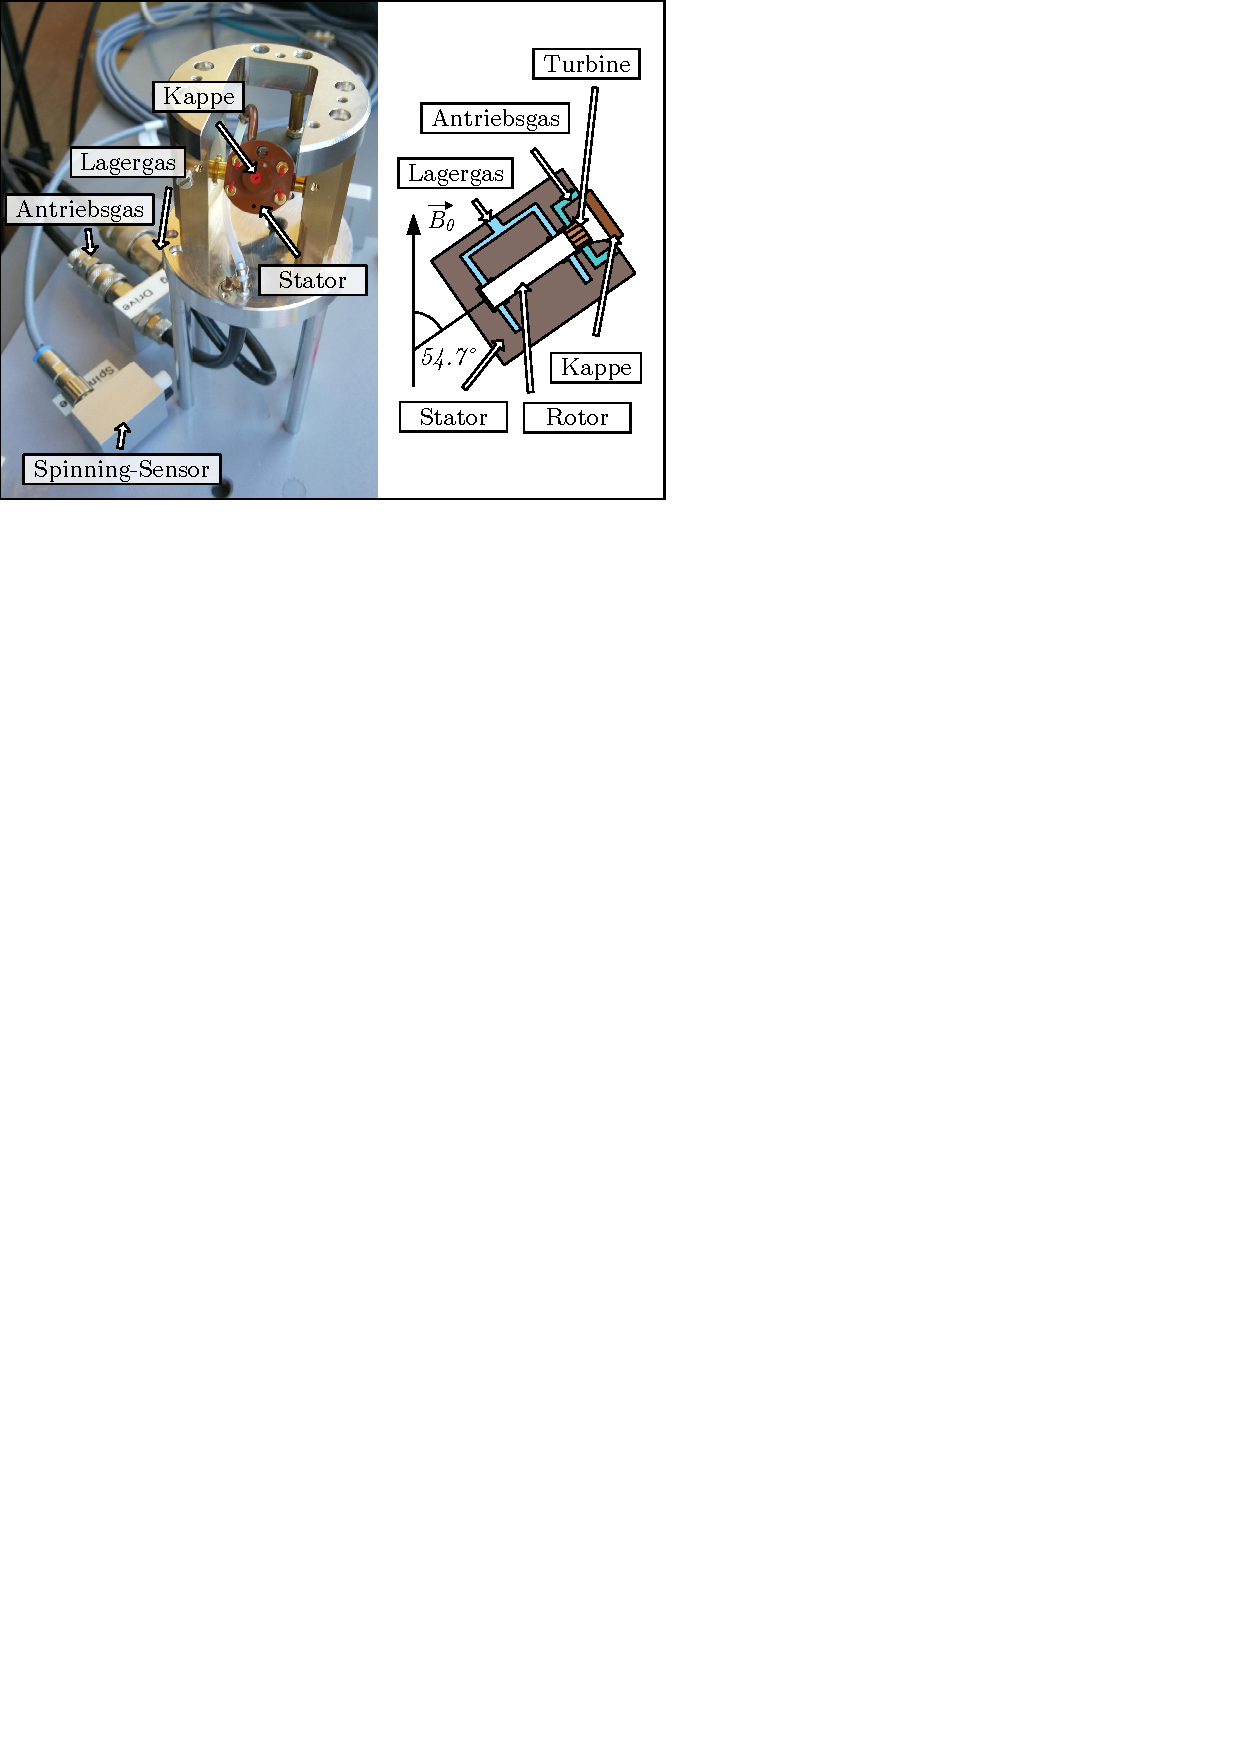
\includegraphics[trim={0cm 21.2cm 9.7cm 0},clip,width=7cm]{images/Device_3.pdf}
			\captionof{figure}{Magic-Angle-Spinning (MAS) Aufbau}
			\label{fig:device3}
			\vspace*{0.5mm}
		\end{Figure}
	
	\subsubsection{Vergleichsspannung}



bbb

\vbox{\hbox{Two lines}\hbox{of type.}}

%\demobox{Das ist ein Test}

%\fbox{Das ist ein Test}

\section{Diskussion}

ccc

